\documentclass{article}

% \usepackage[latin1]{inputenc}
\usepackage[french]{babel}
\usepackage[T1]{fontenc}

\usepackage{lastpage}
\usepackage{fancyhdr}
\usepackage{graphicx}
\usepackage{pdflscape}

\usepackage[a4paper, margin=2.2cm, footskip=12.3pt]{geometry}

\setcounter{secnumdepth}{0}

\newcommand{\header} {
    \setlength{\headheight}{30pt}\pagestyle{fancy}
    \fancyhead[L]{
\includegraphics[height=20pt]{../logo.pdf}}\fancyhead[C]{}
    \fancyhead[R]{Vitória Cosmo, Aubry Mangold, Eva Ray\\\today}\fancyfoot[C]{}
    \fancyfoot[R]{Page \thepage~sur \pageref{LastPage}}\renewcommand{\footrulewidth}{0.3pt}
}

\title{Gestion d'un service de réparation d'objets\\[1ex]Modélisation relationnelle}
\author{Vitória Cosmo, Aubry Mangold, Eva Ray}
\date{22 novembre 2023}

\begin{document}
\header


\maketitle

\pagebreak
\begin{landscape}
\begin{figure}[!htb]
        \centering
        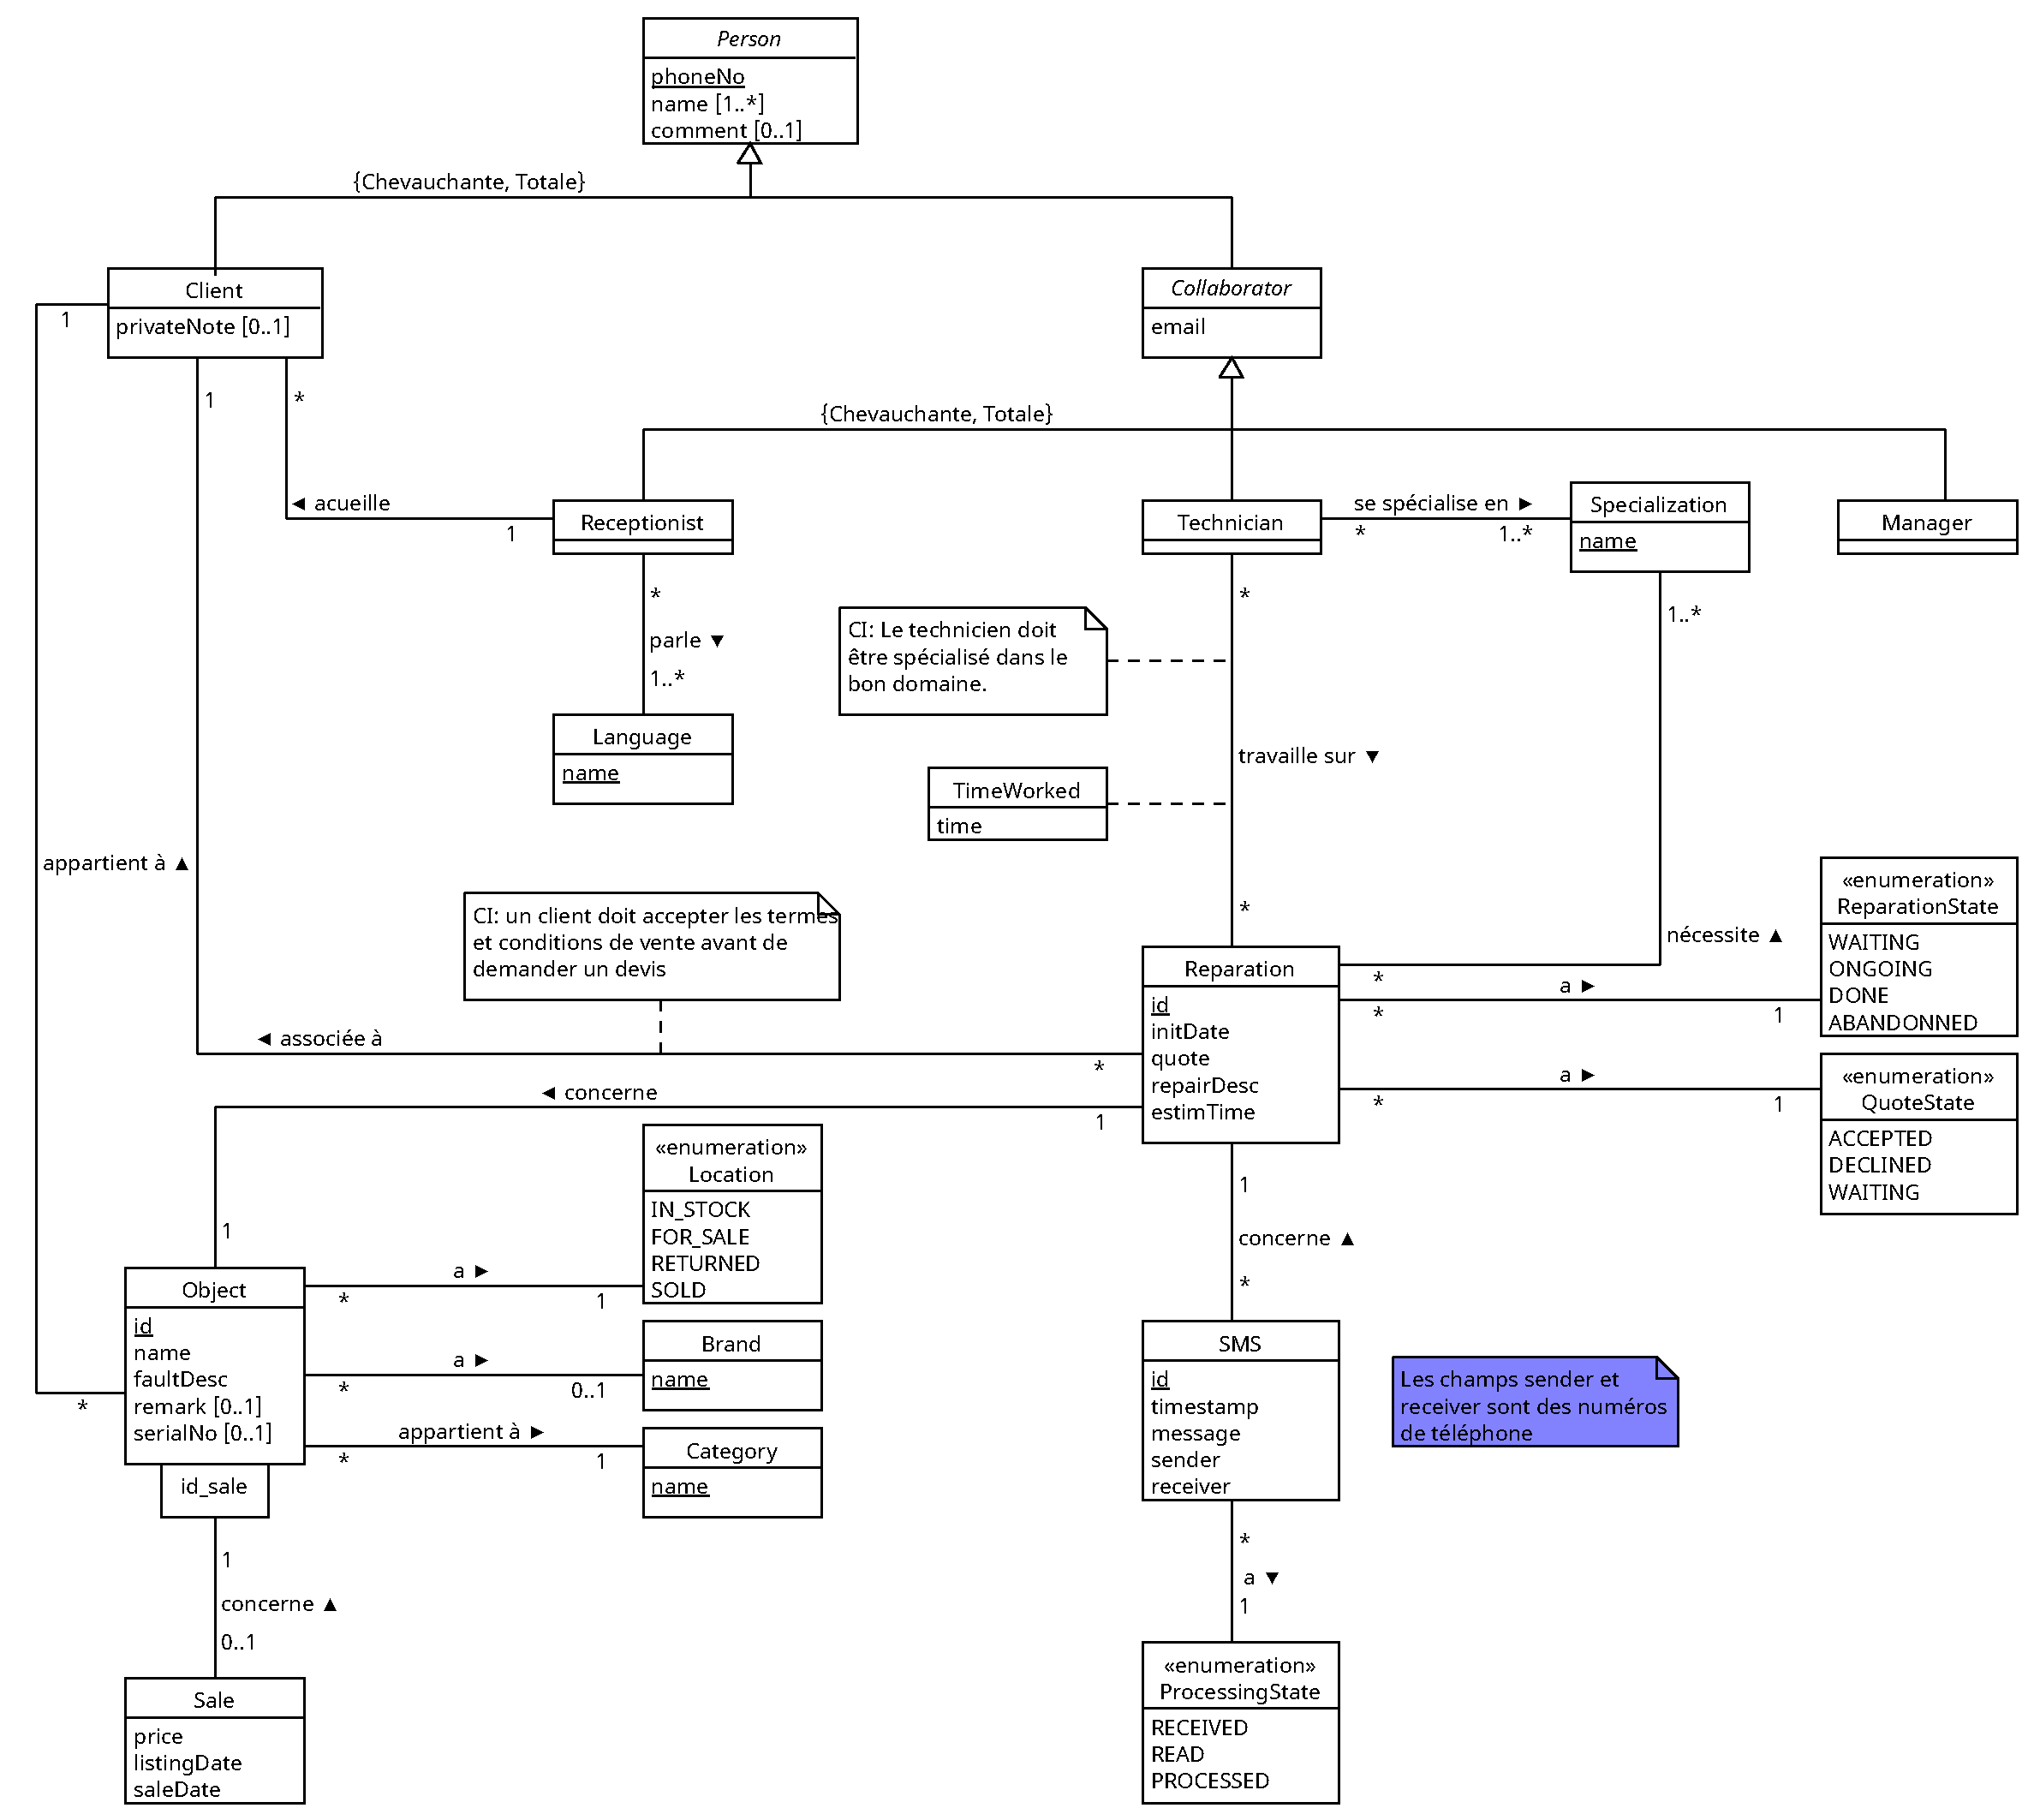
\includegraphics[height=0.93\textheight]{../assets/uml.pdf}
        \caption{Schéma relationnel de la base de données.}
\end{figure}
\end{landscape}

\end{document}